\section{A Brief Survey of Automated Machine Learning}\label{sec:dttts.survey}

Although the focus of this chapter is \gls{hpo}, it is worth mentioning that \gls{hpo} has gradually extended to more general \gls{automl}, for whom the goal is to optimize the entire machine learning pipeline from data preparation to model learning (see e.g.~\citealt{feurer2015fms}). This effort has led to the development of a wide variety of efficient
\gls{automl} systems in the past few years~\citep{thornton2013autoweka,kotthoff2017autoweka,olson2019tpot,mohr2018automl,rakotoarison2019mcts}.

In this section, we give a brief introduction of \gls{automl} and we pay particular attention, of course, to \gls{hpo}. 

We first provide a full-stack pipeline for an \gls{automl} procedure as displayed in Figure~\ref{fig:automl} followed by a general taxonomy on different components of \gls{automl}~\citep{hutter2019automl,zoller2019automl,he2019automl}. 
%We pay particular attention to hyper-parameter optimization, neural architecture search and meta learning later in separate subsections.

\begin{figure}[ht]
    \centering
    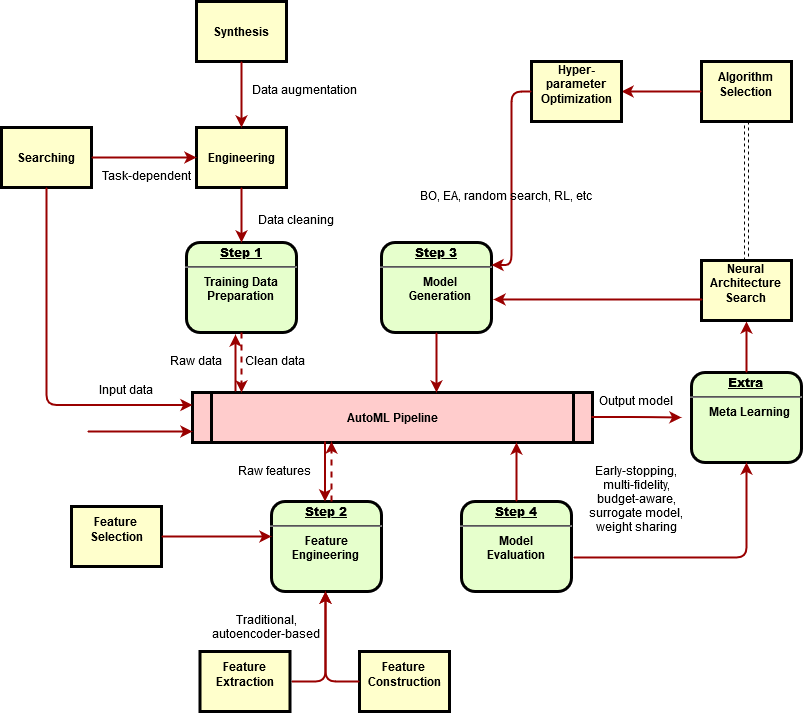
\includegraphics[width=\textwidth]{Chapter6/img/automl.png}
    \caption{The full-stack pipeline of a machine learning task.}
    \label{fig:automl}
\end{figure}


\subsection{The AutoML taxonomy}\label{sec:dttts.survey.taxonomy}

\paragraph{Data preparation.}
The very first step of a machine learning pipeline consists of collecting and preparing clean data.

Data collection often relies on web searching. However, data could be ill-labeled or inaccurate, thus semi-supervised or self-labeling methods are required. When not enough data are available, data synthesis is needed, mainly with the help of data augmentation.

On the other hand, data cleaning is more or less standardized. Typical tricks include normalization, scaling, binarization of numerical (discrete or continuous) attributes, one-hot encoding for categorical attributes, imputation (e.g. with mean values), etc.

\paragraph{Feature engineering.}
Once the data are collected and tidied, the next step is dealing with the features. Depending on the task, feature manipulation can contain three different aspects.

Sometimes we need to reduce irrelevant or redundant features, thus builds a more compact feature subset. This is feature selection. A typical feature selection process starts with subset generation using some (random) search strategy like simulated annealing, genetic algorithms, etc; followed by subset evaluation with filter methods, wrapper methods or embedded methods such as deep neural networks, decision trees, etc; and finally ends up with a validation step.

Another similar but not completely same trick is feature extraction. Feature extraction aims at extracting more informative features using dimensionality reduction techniques like \PCA, \ICA, \LDA, etc. Recent autoencoder-based methods can be used as well.

Finally, we can also construct new features from the raw data to enhance the robustness and generalizability of the model. Typical methods of feature construction include searching methods such as tree-based approaches, genetic algorithms; and annotation-based approaches.

\paragraph{Pipeline generation.} 
The previous two parts are not the focus of this chapter. We are more interested in the third step, namely pipeline generation. Indeed \gls{hpo} is one of the main research topics in this domain.

The pipeline generation is sometimes modeled as a \gls{fms} or \gls{cash} problem, that is typically composed of a model/algorithm selection process and a \gls{hpo} process. We focus on \gls{hpo} in this thesis. It is worth noting, however, that many \gls{hpo} algorithms can also be applied on the full model selection problem as a whole.

A particular instance of \gls{fms} or \gls{cash} is the \gls{nas} problem. \gls{nas} is specific to large modern neural-network models and has become a very hot topic recently (see e.g.~\citealt{elsken2019nas,zoph2018nas,kandasamy2018nas,liu2019darts}). \gls{nas} can also be regarded as a \gls{hpo} problem sometimes, but more often, we can make use of extra information from its inner structure. Anyhow, it is also out of the scope of this manuscript.

\paragraph{Model evaluation and estimation.}
Last but not least, an evaluation of the model is needed at the end. The classic way of evaluating a model is to wait until the completion of the training before assessing its performance on a validation set. Recent work (see e.g.~\citealt{li2017hyperband}) suggests that using a multi-fidelity estimation~\citep{huang2006multifidelity,wu2019multi-fidelity,peherstorfer2018multifidelity} can tremendously reduce the time and resource consumption. Multi-fidelity methods estimate the target function by low-resolution approximations (using only a subset of data for example).

Other methods exist as well that aim at increasing the efficacy of model evaluation and estimation, such as early-stopping, surrogate model, weight sharing, etc. They are mostly specifically designed for \gls{dl} though.
    
%\paragraph{Existing (open source) AutoML frameworks} 
%TPOT, AutoKeras, auto-sklearn, Transmogrif, MLBox

\subsection{Hyper-parameter optimization}\label{sec:dttts.survey.hpo}

We stress again that we only study \gls{hpo} in this chapter. In particular, we do not take care of the model evaluation part, but rather focus on designing efficient model selection algorithms. That being said, we always consider complete training in this thesis, and we do not restrict ourselves to \gls{dl}.

Two naive but daily-used \gls{hpo} methods are \Grid and \Random. More sophisticated model-free methods address \gls{hpo} as a sequential resource allocation problem, by adaptively choosing the next hyper-parameter(s) to explore, based on the results obtained previously. For example, evolutionary optimization follows a process inspired by the biological concept of evolution, which repeatedly replaces the worst-performing hyper-parameter configurations from a randomly initialized population of configurations (see e.g.~\citealt{loshchilov2016cmaes}) for an example of using \CMAES for hyper-parameter tuning. A major drawback of evolutionary optimization is its lack of theoretical understanding.

Model-based approaches also exist. For example, Bayesian optimization is an approach that leverages the sequential nature of the setting. \gls{bo} depends on a prior belief for the target function, typically a Gaussian process. This prior distribution can be updated to a posterior given a sequence of observations. Several algorithms exploiting this posterior distribution to decide where to sample next have been given (see e.g.~\citealt{shahriari2016loop}, for a survey). \citet{snoek2012spearmint} and \citet{klein2017robo} provide Python packages called \Spearmint\ and \RoBO\ to perform hyper-parameter tuning with \gls{bo} methods. Similar packages are available for \PyTorch\ (\BoTorch\footnote{\url{https://botorch.org/}}) and \TensorFlow\ (\flow\ by~\citealt{knudde2017gpflowopt}). Among \gls{bo} algorithms, \TPE~\citep{bergstra2011tpe} and \SMAC~\citep{hutter2011smac} were specifically proposed for \gls{hpo}. A shortcoming of \gls{bo} is that most algorithms select where to sample next based on optimizing some \emph{acquisition function} computed from the posterior, e.g., the expected improvement~\citep{jones1998ei}. This auxiliary task cannot be solved analytically but needs to be performed itself by optimization procedures as \LBFGS that make the process slow. %although this function is usually more regular than the target function. 

% \paragraph{Gray-box optimization}

% \begin{itemize}
%     \item Multi-fidelity Optimization
%     \begin{itemize}
%         \item Bandit-based algorithm \Hyperband, that introduces the concept of partial training;
%         \item `Auto-WEKA` appears to be the only paper that uses only one or a few of the cross-validation folds;
%         \item Bayesian optimization + partial training = \BOHB;
%         \item Learning curve.
%     \end{itemize}
%     \item Gradient-based
% \end{itemize}

% - Current Benchmark (they are mostly designed for a continuous search space)
%     - `Random Search`
%     - `CMA-ES`
%     - `SMAC`
%     - `TPE`
%     - `Hyperband`
%     - `BOHB`

% \subsection{Meta learning}\label{sec:dttts.survey.meta}

% \subsection{Neural architecture search}\label{sec:dttts.survey.nas}

% \paragraph{Model generation}

% \begin{itemize}
%     \item Elemental operations
%     \begin{itemize}
%         \item Convolution;
%         \item Pooling (max-pooling, average-pooling, attention);
%         \item Concatenation;
%         \item Addition;
%         \item Skip connection (ResNet).
%     \end{itemize}
%     \item Model structures
%     \begin{itemize}
%         \item Entire structure;
%         \item Cell-based structure (normal cell or reduction cell like `NASNet`): internal cell design with human-designed operations;
%         \item Progressive structure;
%         \item Morphism-based structure.
%     \end{itemize}
% \end{itemize}

% \paragraph{Hyper-parameter Optimization}

% \begin{itemize}
%     \item Classical HPO methods
%     \item RL-based methods
% \end{itemize}
